\documentclass[10pt,a4paper,notitlepage]{article}

\usepackage[left=1.5cm,text={18cm, 25cm},top=2.5cm]{geometry}
\usepackage{color}
\usepackage[czech]{babel}
\usepackage[T1]{fontenc}
\usepackage[utf8]{inputenc}
\usepackage{listings}
\usepackage{graphicx}
\usepackage{amsthm}
\usepackage{capt-of}
 
\newcommand{\myUrl}[1]{{\color{blue}{#1}}}
\newcommand{\myuv}[1]{\quotedblbase #1\textquotedblleft}
\newcommand{\tab}[1]{\hspace{.2\textwidth}\rlap{#1}}
\newcommand{\bigO}{\ensuremath{\mathcal{O}}}%

\author{Michal Šrubař\\xsruba03@stud.fit.vutbr.cz}
% date s prazdnym argumentem zpusobi neuvedeni date v titulku
\date{\today}	
\title{Paralelní a distribuované algoritmy - Mesh multiplication}

\begin{document}

\maketitle

\section{Zadání}
Pomocí knihovny Open MPI implementujte v~jazyce C++ algoritmus Mesh Multiplication. 

\subsection{Vstup a výstup programu}
Vstupem jsou textové soubory \textit{mat1} a \textit{mat2}.  Výsledná matice,
která je získána operací vynásobením těchto matic je vypsána na standardní
výstup ve formátu specifikovaném níže.

Jako oddělovač čísel na řádku je použita mezera, jako oddělovač jednotlivých
řádků pak znak nového řádku. Výstupem programu je opět matice, která na prvním
řádku obsahuje \textit{radky:sloupce} a na dalších poté výslednou matici, kde
jednotlivé řádky jsou odděleny znakem nového řádku a jednotlivé hodnoty
mezerami.

\section{Pipeline merge sort}
Algoritmus pipeline merge sort pracuje s~lineárním polem procesorů, které jsou
propojeny dvěma kanály s~nenulovou kapacitou. Tato architektura je zobrazena na
obrázku \ref{pic:3}, kde každý procesor očekává na svých vstupních kanálech dvě
posloupnosti, které spojí do výstupní \textbf{seřazené} posloupnosti na svém horním
kanálu a poté vezme další dvě posloupnosti a spojí je do seřazené posloupnosti
na svém dolním kanále. Takto to procesor pořád střídá, dokud je splněna podmínka
práce procesoru.

\begin{figure}[h]
	\centering
	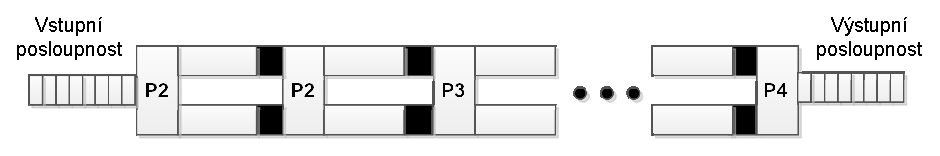
\includegraphics{pms-arch.eps}
  \label{pic:3}
\end{figure}

%FIXME: add pictureo

Aby mohl procesor pracovat, pak musí mít na jednom svém vstupu úplnou
posloupnost a na druhém alespoň jeden prvek. Vyjímku tvoří první procesor, který
pouze předává prvky ze \textbf{vstupní neseřazené posloupnosti} na své výstupní
kanály. Každý procesor začíná předávat nejprve na horní kanál, poté na dolní,
poté na horní atd. Důležité je zmínit, že procesor spojuje vždy pouze ty prvky
které patří do \textbf{stejné posloupnosti}. Výsledkem spojení dvou posloupností
je poté posloupnost dvojnásobné délky.

Nechť \textit{n} je počet prvků vstupní neseřazené posloupnosti, pak počet
procesorů, s~kterými bude algoritmus pracovat, vyjádřuje vztah \ref{pn}:
\begin{equation} \label{pn}
  p(n) = \log_{2}n+1
\end{equation}
 
\subsection{Příklad}
Nechť \textit{X=\{124, 86, 242, 157\}} je řazená posloupnost, pak řazení, které
je demonstrováno na obrázku \ref{pic:2}, budou dle vztahu \ref{pn} provádět tři
procesory a řazení může proběhnou následovně:

%FIXME: číslovat ty procesory od 1!
\begin{enumerate}
  \item Na začátku má procesor P1 ve své vstupní frontě posloupnost \{124, 86, 242, 157\}.
  \item Procesor P1 vezme ze vstupní posloupnosti první prvek s~hodnotou 124 a pošle jej
    horním kanálem procesoru P2. Poté pošle procesoru P2 druhý prvek s~hodnotou 86 přes
    dolní kanál.  Procesor P2 má na svém vstupu dvě posloupnosti a může tedy
    pracovat. Provede porovnání hodnot 124 a 86 a větší z~nich pošle procesoru
    P3 pomocí horního kanálu. Mezi tím procesor P1 posílá třetí prvek s~hodnotou 242,
    který ovšem patří do další posloupnosti.
  \item Procesor P2 teď sice má na svých vstupních kanálech dvě hodnoty, ale
    nemůže je porovnat, jelikož nejsou ze stejné posloupnosti. Nejprve musí
    dokončit porovnávání první posloupnosti, což znamená odeslat hodnotu 86
    procesoru P3.  Procesor P1 může zároveň poslat procesoru P2 poslední hodnotu
    , tj. 157.
  \item Až nyní procesor P2 splňuje podmínku a může porovnat hodnoty 242 a 157,
    jelikož jsou ze stejné posloupnosti. Větší hodnotu, tj. 242, pošle procesoru P3.
  \item Procesor P3 může hned porovnat přijatou hodnotu 157 s~hodnotou 124 a
    větší z~nich zařadit do výstupní posloupnosti.
  \item Na dolní kanál procesoru P3 již nepřijde žádný prvek, takže může
    zkopírovat seřazenou posloupnost z~horního kanálu do výstupní fronty čímž
    dostáváme výslednou seřazenou posloupnost \textit{Y=\{86,124,157,242\}}.
\end{enumerate}

\begin{figure}[h]
	\centering
	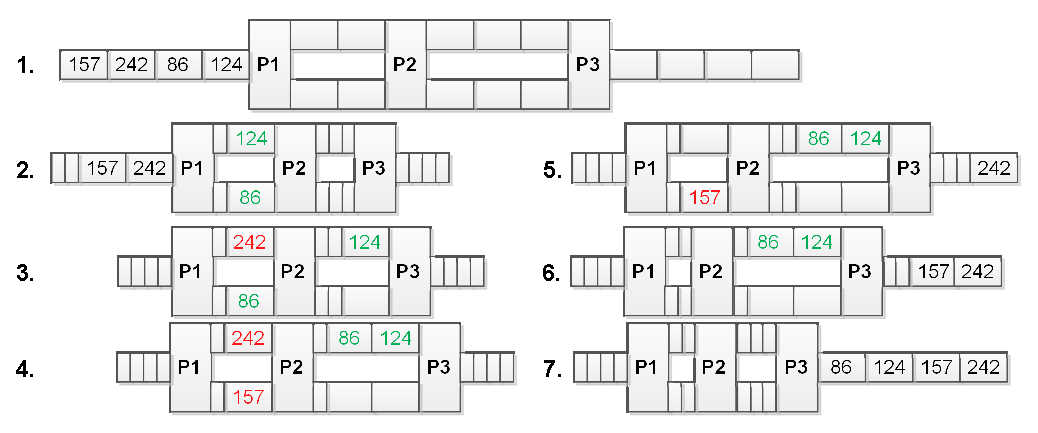
\includegraphics{prl-pms.eps}
  \label{pic:2}
\end{figure}

\subsection{Analýza}\label{analyza}
Procesor P2 začne pracovat až 2 cykly po procesoru P1, jelikož procesor P1 musí
nejprve poslat prvek ze vstupní posloupnosti na horní kanál a poté na dolní
kanál. Procesor P3 poté začne pracovat až 3 cykly za procesorem P2, protože P2
nejprve pošle jednu seřazenou posloupnost na horní kanál a poté musí poslat
alespoň jeden prvek z~druhé seřazené posloupnosti a až poté muže procesor P3
začít pracovat.

Obecně tedy platí, že procesor $P_{i}$ může začít pracovat až v~okamžiku, kdy se
na jednom jeho vstupu nachází posloupnost délky $2^{i-2}$ a na druhém posloupnost
délky 1. Procesor $P_{i}$ pak tedy začne pracovat $2^{i-2}+1$ cyklů po procesoru
$P_{i-1}$.

Procesor $P_{i}$ obecně začne pracovat v~cyklu: $$2^{i-1}+i-1$$ a skončí
v~cyklu:
$$(n-1)+2^{i-1}+i-1$$ kde n je počet řazených prvků vstupní posloupnosti.
Celý algoritmus poté skončí za $2n+\log_{2}n-1$ cyklů. Časová složitost se skládá
z~lineární a logaritmické složky a jelikož je logaritmická pro tu lineární
zanedbatelná, pak celková časová složitost je lineární a tedy $t(n) = \bigO(n)$.
Cena algoritmu je poté $c(n) = t(n) * p(n) = \bigO(n) * (\log_{2}n+1) =
\bigO(n*\log{n})$. Cena tedy je optimální.

\section{Implementace}
Algoritmus je implementován v~jazyce C s~využitím knihovny OpenMPI\footnote{Open
Message Passing Interface, http://www.open-mpi.org}, kde jednotlivé procesory jsou
simulovány procesy operačního systému. Kapacita kanálů jednotlivých procesorů je
realizována pomocí linuxových front\footnote{http://linux.die.net/man/3/queue},
kde každý procesor má svoji horní a dolní vstupní frontu kromě prvního
procesoru, který pracuje pouze se vstupní frontou, kde jsou před samotným
začátkem algoritmu načteny vstupní hodnoty ze souboru \texttt{numbers}.
Poslední procesor má poté navíc ještě výstupní frontu kam ukládá prvky výstupní
seřazené posloupnosti.

\subsection{Sekvenční diagram}
Nechť $X=\{x_{1}, x_{2}, x_{3}, \dots, x_{m}\}$ je řazená posloupnost a $N$
reprezentuje počet procesů, pak sekvenční diagram, který je zobrazen na obrázku \ref{pic:3}, popisuje komunikaci
mezi procesy P1 až PN. První proces P1 prochází svoji vstupní frontu a předává z~ní
řazené položky jednu za druhou dalšímu procesu, tj. P2, pomocí blokujícího
rozhranní
\textit{MPI\_Send}\footnote{https://www.open-mpi.org/doc/v1.8/man3/MPI\_Send.3.php}.
Jak bylo popsáno v~sekci \ref{analyza}, proces P2 začne pracovat až dva cykly po
procesu P1 jelikož musí počkat, až obě jeho vstupní fronty budou obsahovat hodnoty
ze stejné posloupnosti.

Jakmile má proces splňuje podmínku práce, tak porovná
první prvek z~horní a dolní fronty a větší z~nich posílá svému pravému
sousedovi. Poslední proces PN taktéž provádí porovnávání prvků, ale větší z~nich
již neposílá pravému sousedovi, ale ukládá je do své výstupní fronty, kde se po
skončení algoritmu nachází seřazená posloupnost $Y=\{y_{1}, y_{2}, y_{3}, \dots,
y_{m}\}$.  Každý procesem tak projde každý prvek z~řazené posloupnosti.  

\begin{figure}[h]
	\centering
  \scalebox{0.85}{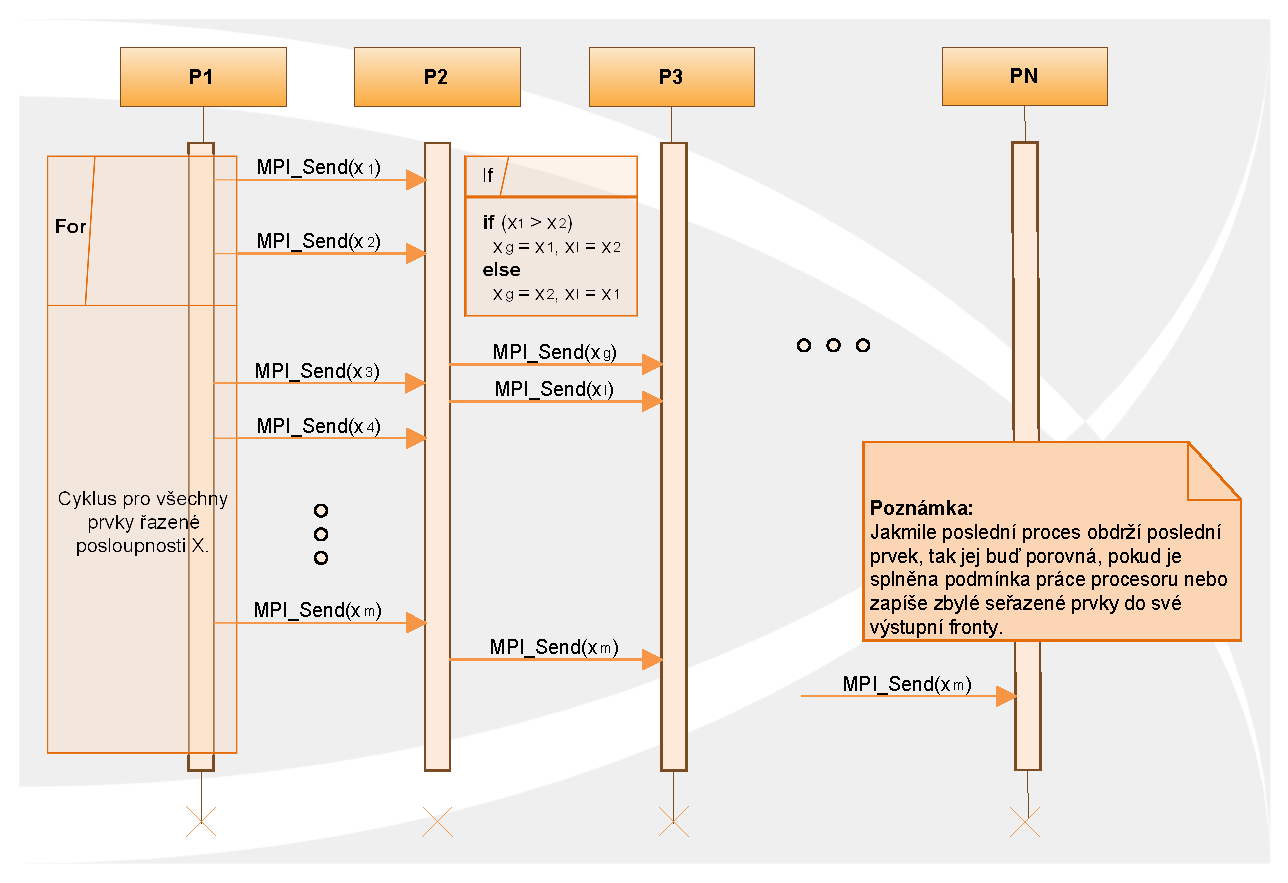
\includegraphics{prl.eps}}
  \label{pic:3}
  \caption{Sekvenční diagram komunikace mezi procesy.}
\end{figure}

\subsection{Výsledky experimentování}
Pro měření doby práce algoritmu byla využita funkce
\textit{clock\_gettime()}\footnote{http://linux.die.net/man/3/clock\_gettime}.
Při experimentech byl měřen pouze čas algoritmu a ne načítání vstupní
posloupnosti ze souboru a výstup výsledků na terminál. Měření proběhlo pro
vstupní posloupnosti o~délkách 2, 4, 8, 16, 32, 64 a 128 prvků. Pro každou délku
bylo vygenerováno celkem 100 různých vstupních posloupností ze kterých poté byla spočtena
průměrná doba trvání algoritmu pro konkrétní délku vstupní posloupnosti.

Testování proběhlo na serveru \textit{merlin.fit.vutbr.cz} pomocí skriptu
\textit{performance\_test.sh}, jehož výsledky zobrazuje tabulka \ref{exp:res} a
obrázek \ref{fig:1}, kde sloupec n reprezentuje délku vstupní posloupnosti a čas
je průměrný čas v~nanosekundách.

\begin{figure}[h]
\centering
\begin{minipage}[t]{.4\textwidth}
\centering
\vspace{0pt}
  \input{introduction}
\caption{Grafické zobrazení naměřených výsledků.}
\label{fig:1}
\end{minipage}\hfill
\begin{minipage}[t]{.4\textwidth}
\centering
\vspace{0pt}

\caption{Výsledky.}
  \begin{tabular}{|c|c|}
    \hline
  \textbf{n} & \textbf{čas [ns]} \\ \hline
    2 &   76099\\ \hline
    4  &  101573\\ \hline
    8   & 142423\\ \hline
    16 &  197219\\ \hline
    32 &  304561\\ \hline
    64 &  636753\\ \hline
    128 & 1273051\\ \hline
  \end{tabular}
\label{exp:res}
\end{minipage}
\end{figure}

\section{Závěr}
Cílem tohoto projektu bylo popsat, analyzovat, implementovat a otestovat
algoritmus pipeline merge sort. V~sekci \ref{analyza} bylo odvozeno, že
algoritmus má lineární složitost, což bylo potvrzeno pomocí provedeného
experimentu jehož výsledky zobrazuje graf na obrázku \ref{fig:1}.
Časová složitost ani nemůže být lepší, jelikož pracujeme s~lineárním polem
procesorů a výsledná seřazená posloupnost se musí objevit na výstupu posledního
procesoru.

\end{document}
